\documentclass[conference]{IEEEtran}
\IEEEoverridecommandlockouts
% The preceding line is only needed to identify funding in the first footnote. If that is unneeded, please comment it out.
\usepackage{cite}
\usepackage{amsmath,amssymb,amsfonts}
\usepackage{algorithmic}
\usepackage{graphicx}
\usepackage{textcomp}
\usepackage{xcolor}
\usepackage{url}
\usepackage{subfigure}


\usepackage{soul} % Para resaltar texto
\newcommand{\highlight}[1]{\colorbox{yellow!50}{#1}} % Comando personalizado para fondo amarillo

\def\BibTeX{{\rm B\kern-.05em{\sc i\kern-.025em b}\kern-.08em
		T\kern-.1667em\lower.7ex\hbox{E}\kern-.125emX}}

\begin{document}
	
	\title{Implementación de sistema de clarificación automatizado para potabilización de efluentes contaminados}
	
	\author{
		\IEEEauthorblockN{1\textsuperscript{st} Asunci\'on Cordero}
		\IEEEauthorblockA{\textit{Universidad Aut\'onoma del Carmen} \\
			Ciudad del Carmen, Campeche, M\'exico \\
			acordero@pampano.unacar.mx}
		\and
		\IEEEauthorblockN{2\textsuperscript{nd} Luis Medina}
		\IEEEauthorblockA{\textit{Universidad Tecnol\'ogica y Politécnica} \\ \textit{del Valle del Carrizo} \\
			Cd. L\'opez Mateos, M\'exico \\
			luismedina@utpvalledelcarrizo.edu.mx}
		\and
		\IEEEauthorblockN{3\textsuperscript{rd} Adelina Martinez}
		\IEEEauthorblockA{\textit{Instituto Tecnol\'ogico de Oaxaca} \\
			Oaxaca de Juárez, Oax, M\'exico \\
			adelina.martinez@itoaxaca.edu.mx}
		\and
		\IEEEauthorblockN{4\textsuperscript{th} Alejandro Baños}
		\IEEEauthorblockA{\textit{Instituto Tecnol\'ogico Latinoamericano} \\
			Córdoba, Veracruz, M\'exico \\
			alejandro.banos@itl.edu.mx}
		\and
		\IEEEauthorblockN{5\textsuperscript{th} Federico Arias}
		\IEEEauthorblockA{\textit{Inst. Tecnol\'ogico Superior de Zapopan} \\
			Zapopan, Jalisco, M\'exico \\
			federico.arias@itszapopan.edu.mx}
		\and
		\IEEEauthorblockN{6\textsuperscript{th} Israel Viveros}
		\IEEEauthorblockA{\textit{Inst. Tecnol\'ogico Superior de Alvarado} \\
			Alvarado, Veracruz, M\'exico \\
			israel.vt@alvarado.tecnm.mx}
	}
	
	\maketitle
	
	\begin{abstract}
	El acceso a agua potable representa uno de los principales retos de sostenibilidad en el siglo XXI, especialmente en comunidades marginadas donde los recursos tecnológicos y económicos son limitados. En este contexto, el presente trabajo propone el desarrollo de un sistema automatizado de clarificación de efluentes contaminados basado en la técnica de coagulación-floculación utilizando Moringa Oleífera como agente natural. A diferencia de los coagulantes sintéticos convencionales, la moringa presenta ventajas como bajo costo, biodegradabilidad y ausencia de toxicidad residual. El diseño del sistema se estructuró bajo un enfoque mecatrónico que integra subsistemas mecánicos, electrónicos y de control, incorporando instrumentación en tiempo real para el monitoreo de parámetros críticos (turbidez, TDS, pH, DBO y DQO).
	
	Metodológicamente, el proyecto adoptó el marco ágil Scrum para gestionar su complejidad interdisciplinaria y garantizar resultados incrementales. Se definieron seis sprints, con entregables funcionales que abarcaron desde el modelado matemático y la simulación del proceso hasta la validación experimental en campo. El plan de métricas incluyó indicadores de calidad del agua conforme a normas oficiales mexicanas, métricas de productividad en el desarrollo del prototipo y métricas de proceso para asegurar eficiencia operativa. Asimismo, se implementaron herramientas digitales para evaluación del software embebido y MATLAB/Simulink para simulación de procesos.
	
	Los resultados preliminares confirman la viabilidad de un sistema autónomo, sostenible y replicable que contribuye al cumplimiento del ODS 6, ofreciendo una alternativa tecnológica de alto impacto social y ambiental.
	
	Index terms: floculación, Moringa Oleífera, tratamiento de agua, Scrum, métricas de calidad, sistemas embebidos.
	
	
	\end{abstract}
	
	\begin{IEEEkeywords}
		Tratamiento de agua, turbidez, \textit{Moringa oleifera}, automatización, sistemas embebidos, sustentabilidad.
	\end{IEEEkeywords}
	
	\section{Introducción}
	El acceso al agua potable constituye uno de los principales desafíos ambientales y sociales del siglo XXI. En México, únicamente el 32\% del agua es renovable y el 10\% del agua dulce disponible se destina al uso doméstico, porcentaje superior al promedio mundial del 8\%, lo que refleja una crisis hídrica latente \cite{b1}. A esta problemática se suma la creciente contaminación de cuerpos acuíferos y mantos freáticos, lo que ha intensificado la necesidad de tecnologías innovadoras y sostenibles para la clarificación y potabilización de aguas residuales.
	
	Una de las técnicas más extendidas para el tratamiento de agua es la coagulación-floculación, que se aplica previamente a procesos físicos como sedimentación o filtración. Tradicionalmente se emplean coagulantes sintéticos a base de sales metálicas, los cuales, si bien resultan efectivos, presentan limitaciones como altos costos, necesidad de conocimientos especializados en su dosificación y riesgos de toxicidad \cite{b2}, \cite{b3}. Estas desventajas han impulsado la búsqueda de alternativas naturales más seguras, económicas y ambientalmente sostenibles.
	
	En este contexto, la semilla de Moringa oleífera se perfila como un floculante orgánico viable, capaz de neutralizar partículas coloidales y facilitar su sedimentación gracias a su contenido de proteínas catiónicas \cite{b4}. Además de su efectividad comparable a los coagulantes sintéticos, este agente natural presenta propiedades antimicrobianas, es inocuo para el consumo humano y genera lodos biodegradables que pueden aprovecharse como fertilizantes \cite{b5}.
	
	El presente trabajo propone el desarrollo e implementación de un dispositivo automatizado que emplee Moringa oleífera como floculante natural, integrando sensores fisicoquímicos, actuadores y un sistema embebido para garantizar un proceso de clarificación eficiente, autónomo y accesible como se muestra esquemáticamente en la figura 1.
	
	\begin{figure}[htbp]
		\centering
		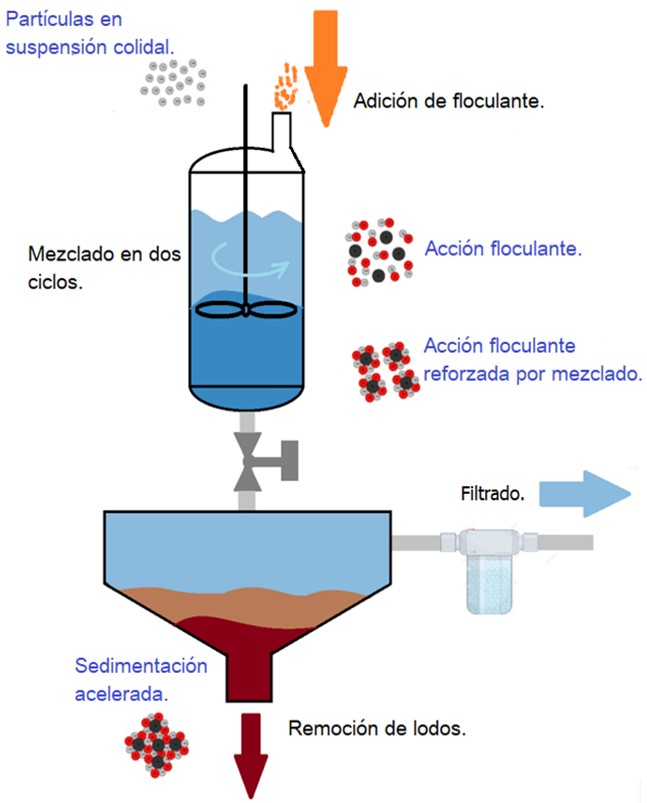
\includegraphics[width=\columnwidth]{fig1.jpg}
		\caption{Etapas físico químicas del proceso de coagulación-floculación}
		\label{fig:esquema-sistema}
	\end{figure}
	
	\section{ PLANTEAMIENTO DEL PROBLEMA}
	
	El tratamiento artesanal de aguas turbias continúa siendo una práctica común en comunidades rurales y zonas marginadas. Dicho enfoque carece de estandarización, depende del conocimiento empírico del operador y no garantiza la inocuidad del agua obtenida. Asimismo, la dependencia de coagulantes sintéticos incrementa los costos de operación y genera riesgos de toxicidad asociados a una dosificación inadecuada \cite{b6}.
	
	De esta forma, la problemática central radica en la ausencia de un sistema autónomo, accesible y sostenible que permita clarificar aguas con turbiedad media o alta mediante el uso de coagulantes naturales.
	
	\section{JUSTIFICACIÓN}
	El desarrollo de un prototipo automatizado controlado mediante software embebido representa una solución innovadora a las limitaciones de los métodos tradicionales tal como se muestra en la figura 2. 
	
	\begin{figure}[htbp]
		\centering
		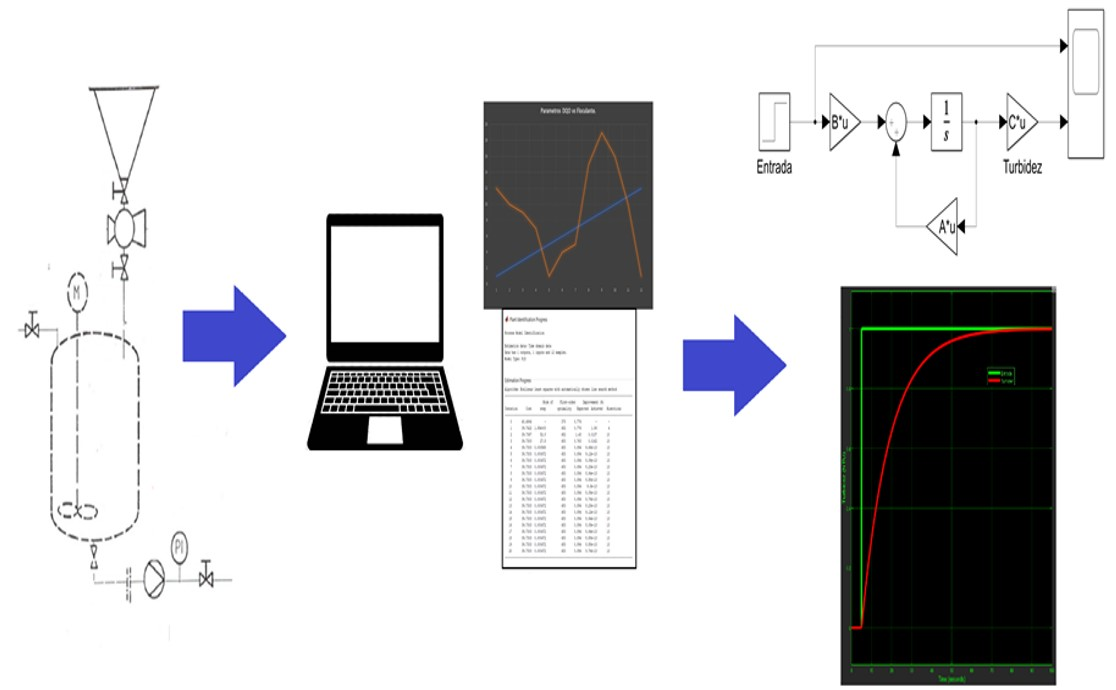
\includegraphics[width=\columnwidth]{fig2.jpg}
		\caption{Análisis de sintonía del controlador, para diseño de planta y datos de salida}
		\label{fig:esquema-sistema}
	\end{figure}
	
	Con base el sistema propuesto se obtiene un dispositivo que permite lograr las siguientes características operativas:
	
	\begin{itemize}
		\item Sustituir procesos manuales por un sistema autónomo de bajo costo.
		
		\item Reducir la dependencia de químicos industriales, empleando un floculante natural, seguro y biodegradable.
		
		\item Integrar sensores de turbidez, pH, sólidos disueltos totales (TDS) y temperatura, para monitorear y regular el proceso en tiempo real.
		
		\item Brindar simplicidad de operación, sin necesidad de conocimientos avanzados en química, lo que facilita su implementación en comunidades de escasos recursos \cite{b7}.
		
	\end{itemize}
	
	El proyecto no solo aporta valor desde una perspectiva técnica ambiental, sino que también promueve la equidad social al facilitar el acceso a agua tratada en zonas vulnerables. Asimismo, se alinea con los Objetivos de Desarrollo Sostenible (ODS), particularmente con el ODS 6: Agua limpia y saneamiento.
	
	\section{Marco metodológico: gestión del proyecto y plan de métricas}
	
	\subsection{Gestión del proyecto}
	
	Para el desarrollo del sistema embebido de tratamiento de efluentes, se adoptó la metodología ágil Scrum, ampliamente reconocida por su capacidad de adaptación en entornos de alta incertidumbre y complejidad \cite{b8}. Esta metodología permite dividir el proyecto en iteraciones llamadas sprints, cada una con entregables funcionales que pueden ser evaluados y ajustados en función de la retroalimentación obtenida \cite{b8}.
	
	El proyecto se estructuró en cinco sprints, alineados con las etapas operativas del prototipo descritas en el documento técnico:
	
	\begin{itemize}
		\item \textbf{Sprint 1:} Integración de sensores y microcontrolador.
		\item \textbf{Sprint 2:} Control de actuadores.
		\item \textbf{Sprint 3:} Interfaz de usuario.
		\item \textbf{Sprint 4:} Algoritmo de operación.
		\item \textbf{Sprint 5:} Validación y pruebas.
	\end{itemize}
	
	La integración antes mencionada se ejemplifica en la figura 3.
	
	\begin{figure}[htbp]
		\centering
		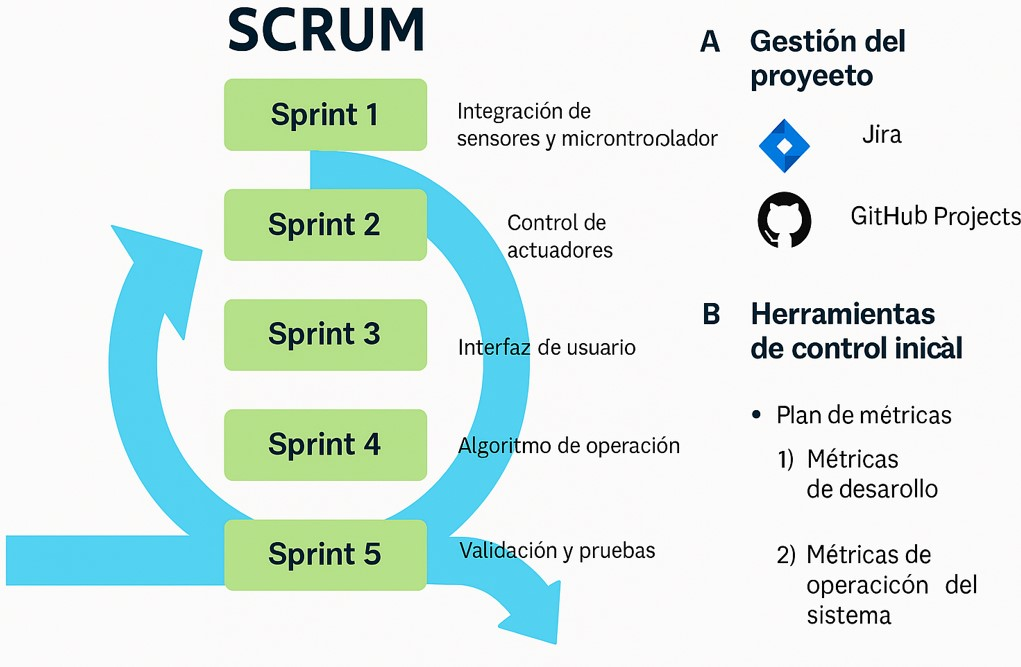
\includegraphics[width=\columnwidth]{fig3.jpg}
		\caption{Implementacion de metodología SCRUM}
		\label{fig:esquema-sistema}
	\end{figure}
	
	\subsection{Herramientas de control inicial}
	
	Para la gestión del proyecto y control de calidad del desarrollo, se implementaron herramientas ampliamente utilizadas en entornos ágiles:
	
	\begin{itemize}
		\item \textbf{Jira:} Permite la planificación de sprints, seguimiento de tareas y generación de informes en tiempo real \cite{b9}.
		\item \textbf{GitHub Projects:} Facilita el control de versiones, colaboración entre desarrolladores y documentación técnica \cite{b9}.
		\item \textbf{SonarQube:} Herramienta de análisis estático que evalúa la calidad del código fuente, detecta errores, vulnerabilidades y proporciona métricas como duplicación, cobertura de pruebas y complejidad ciclomática \cite{b10}.
	\end{itemize}
	
	\subsection{Plan de métricas}
	
	El plan de métricas se divide en dos niveles:
	
	\subsubsection{Métricas de desarrollo}
	
	\begin{itemize}
		\item \textbf{Velocidad del equipo:} Historias de usuario completadas por sprint.
		\item \textbf{Tasa de resolución de errores:} Porcentaje de incidencias resueltas.
		\item \textbf{Cobertura de pruebas:} Porcentaje de código cubierto por pruebas unitarias \cite{b10}.
	\end{itemize}
	
	\subsubsection{Métricas de operación del sistema}
	
	\begin{itemize}
		\item \textbf{Precisión de sensores:} Desviación estándar entre lecturas reales y esperadas.
		\item \textbf{Tiempo de respuesta:} Latencia entre señal de sensor y activación de actuador.
		\item \textbf{Eficiencia de tratamiento:} Reducción porcentual de turbidez, DBO y DQO.
		\item \textbf{Estabilidad del sistema:} Número de ciclos completados sin fallos.
	\end{itemize}
	
	El arreglo de métricas asociados al desarrollo del sistema se muestra en la figura 4.
	
	\begin{figure}[htbp]
		\centering
		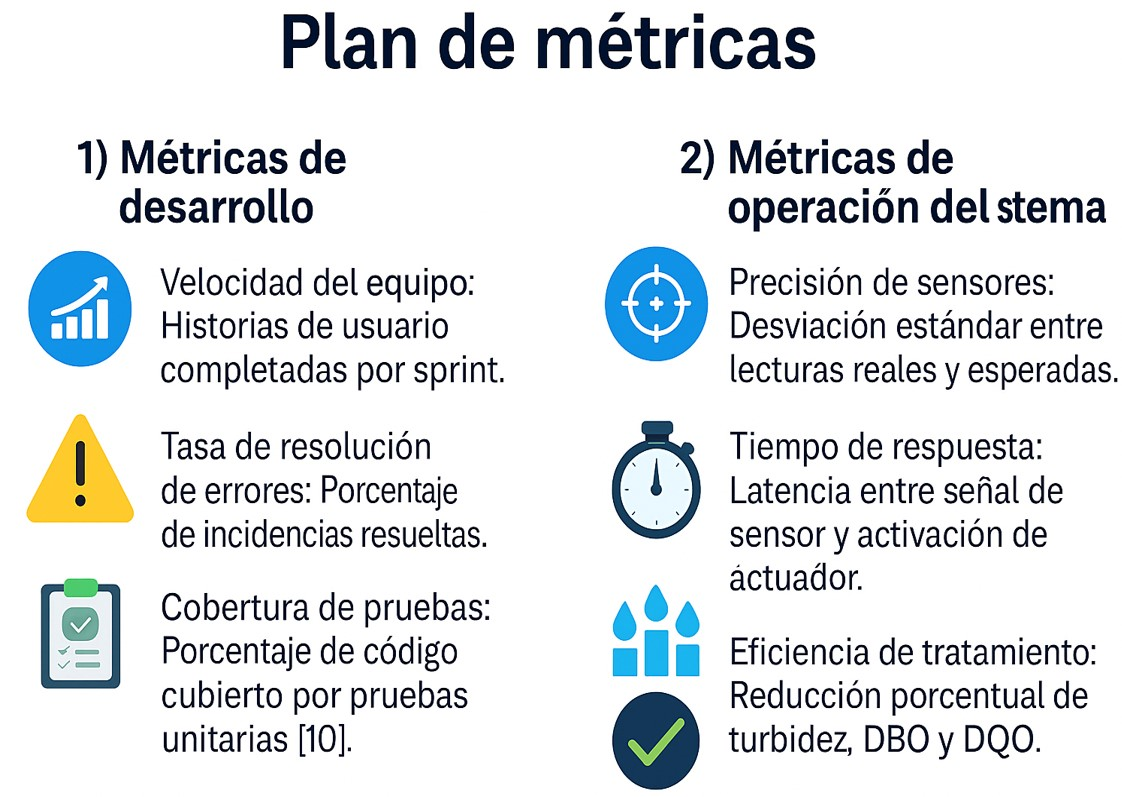
\includegraphics[width=\columnwidth]{fig4.jpg}
		\caption{Implementacion de metricas de alcance}
		\label{fig:esquema-sistema}
	\end{figure}
	
	El desarrollo propone un sistema automatizado de bajo costo y alta fiabilidad \cite{b12}. En este contexto, se plantea un prototipo que integra sensores, actuadores y un controlador embebido, cuyo éxito depende de una planificación precisa de recursos, una adecuada gestión de riesgos y un cronograma robusto \cite{b13}.
	
	La metodología aquí descrita se fundamenta en estándares internacionales, tales como el IEEE Std 830-1998 para especificación de requerimientos \cite{b14}, IEEE Std 1540-2001 para gestión de riesgos \cite{b15}, y la metodología COCOMO para estimación de esfuerzo \cite{b16}.
	
	\section{Estimación de Recursos y Esfuerzo}
	
	\subsection{Técnica de Descomposición}
	
	El sistema se descompuso en cinco módulos principales: adquisición de datos, control embebido, automatización del proceso, interfaz de usuario y validación. Cada módulo se estimó en horas-hombre considerando tareas de diseño, programación, integración y pruebas \cite{b17}. La suma total resultó en 600 horas-hombre ($\sim$3.5 meses con un equipo de dos ingenieros).
	
	\subsection{Estimación mediante COCOMO}
	
	Aplicando el modelo orgánico de COCOMO para un tamaño aproximado de 2.5 KLOC:
	
	\begin{itemize}
		\item Esfuerzo: $E = 2.4 \times (\text{KLOC})^{1.05} \approx 6.4$ personas-mes.
		\item Tiempo de desarrollo: $T = 2.5 \times (E)^{0.38} \approx 5.8$ meses.
	\end{itemize}
	
	Estos valores se alinean con la descomposición, lo que refuerza la validez de la estimación \cite{b16}, \cite{b18}.
	
	\subsection{Decisión: Desarrollar vs. Comprar}
	
	\begin{itemize}
		\item \textbf{Desarrollar:} software embebido y algoritmos de control, por requerir alta personalización.
		\item \textbf{Comprar:} sensores de turbidez, pH y TDS, dado su disponibilidad comercial \cite{b19}.
		\item \textbf{Híbrido:} servoválvulas comerciales modificadas con impresión 3D, reduciendo costos y tiempo de desarrollo \cite{b20}.
	\end{itemize}
	
	\section{Plan de Riesgos}
	
	\subsection{Identificación de Riesgos}
	
	Fallos en sensores, desgaste mecánico de bombas, errores de calibración, interrupciones de energía y riesgos sanitarios por clarificación insuficiente.
	
	\subsection{Proyección y Priorización}
	
	Se aplicó un análisis de probabilidad-impacto \cite{b21}. Los riesgos de sensores presentan probabilidad alta e impacto crítico; los cortes eléctricos, probabilidad baja pero impacto medio.
	
	\subsection{Estrategias Proactivas y Reactivas}
	
	\begin{itemize}
		\item \textbf{Proactivas:} redundancia en sensores, mantenimiento preventivo, simulación previa en MATLAB/Simulink \cite{b22}.
		\item \textbf{Reactivas:} rutinas de auto-limpieza, alarmas visuales y sonoras, sustitución rápida de módulos \cite{b23}.
	\end{itemize}
	
	\subsection{Plan RSGR}
	
	\begin{itemize}
		\item \textbf{Responsable:} equipo de ingeniería.
		\item \textbf{Seguimiento:} bitácora digital de fallas.
		\item \textbf{Gestión:} control de calidad basado en ISO/IEC 25010 \cite{b24}.
		\item \textbf{Recuperación:} protocolos de reemplazo rápido de sensores y restauración de software.
	\end{itemize}
	
	\section{Red de Tareas y Cronograma}
	
	\subsection{Dependencias}
	
	\begin{enumerate}
		\item Requerimientos y diseño conceptual (Semanas 1--2).
		\item Selección de sensores y actuadores (Semanas 3--4).
		\item Simulación y programación inicial (Semanas 4--8).
		\item Ensamble y pruebas de hardware (Semanas 5--9).
		\item Integración hardware-software (Semanas 10--12).
		\item Pruebas de laboratorio (Semanas 13--16).
		\item Ajustes y validación final (Semanas 17--18).
	\end{enumerate}
	
	\subsection{Cronograma Estimado (semanas)}
	
Diseño CAD y simulación: 1--2 (2 Semanas)\\
	Fabricación: 3--5 (2 Semanas)\\
	Integración electrónica: 6--7 (1 Semana)\\
	Programación: 8--10 (2 Semanas)\\
	Pruebas de laboratorio: 11--12 (1 Semana)\\
	Validación en campo: 13--15 (2 Semanas)\\
	Modelado y simulación: 16--17 (1 Semana)\\
	Documentación: 18 (1 Semana)
	
		\vspace{1em}
		
	La anterior planificación para ejecución del Proyecto propuesto se ejemplifica por medio de gráficos de Gantt, como se muestran segmentados en sus diferentes sprints en la figura 5.
	
		
	
	\begin{figure}[htbp]
	\centering
	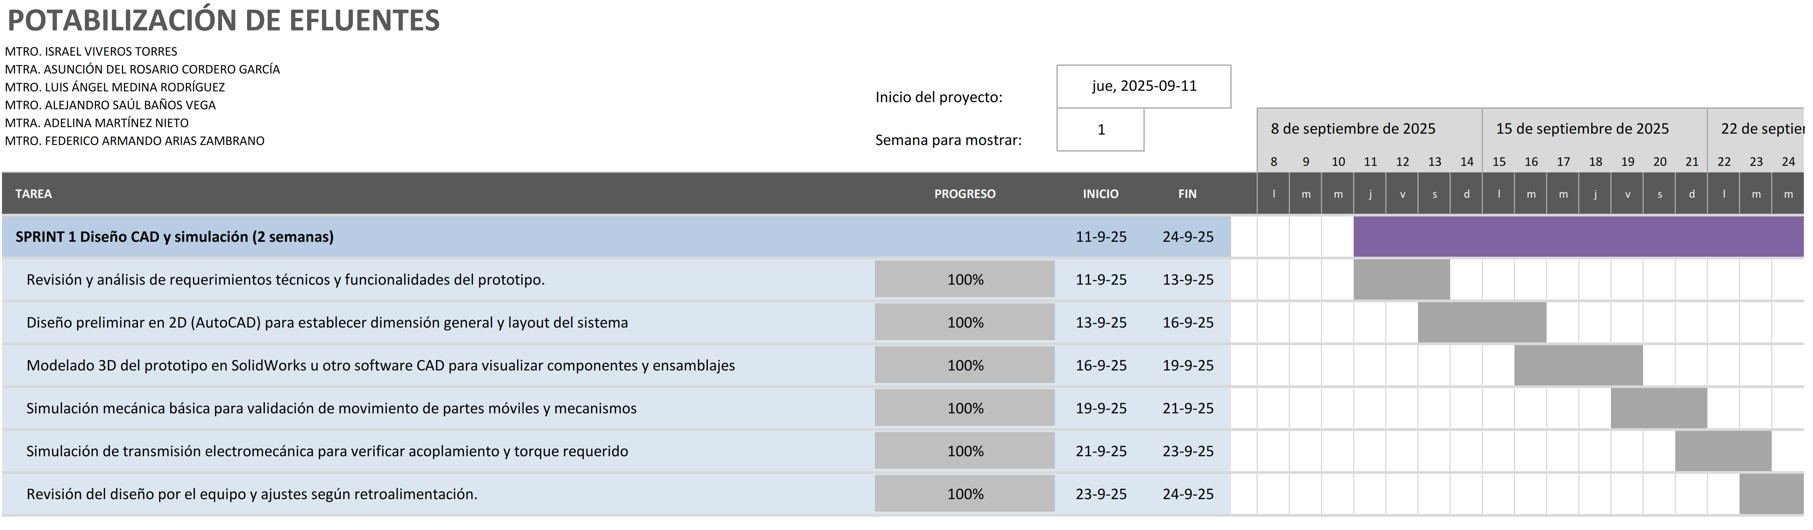
\includegraphics[width=\columnwidth]{fig5_1.jpg}
	%\caption{Implementacion de metricas de alcance}
	%\label{fig:esquema-sistema}
	\end{figure}
	
	\begin{figure}[htbp]
	\centering
	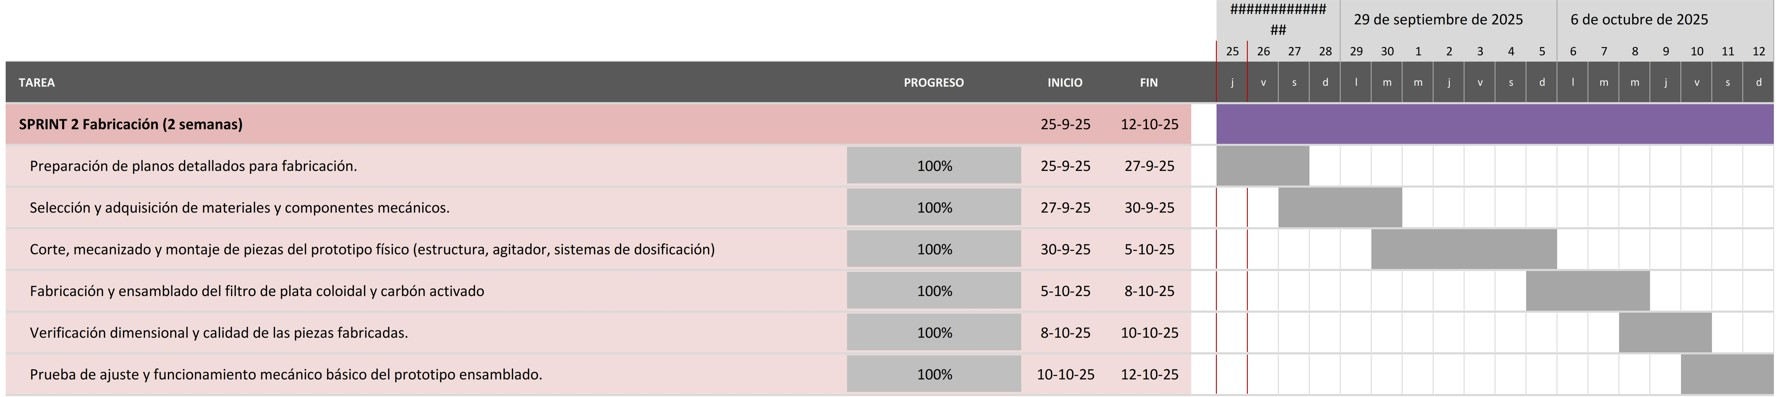
\includegraphics[width=\columnwidth]{fig5_2.jpg}
	%\caption{Implementacion de metricas de alcance}
	%\label{fig:esquema-sistema}
	\end{figure}
	
	\begin{figure}[htbp]
	\centering
	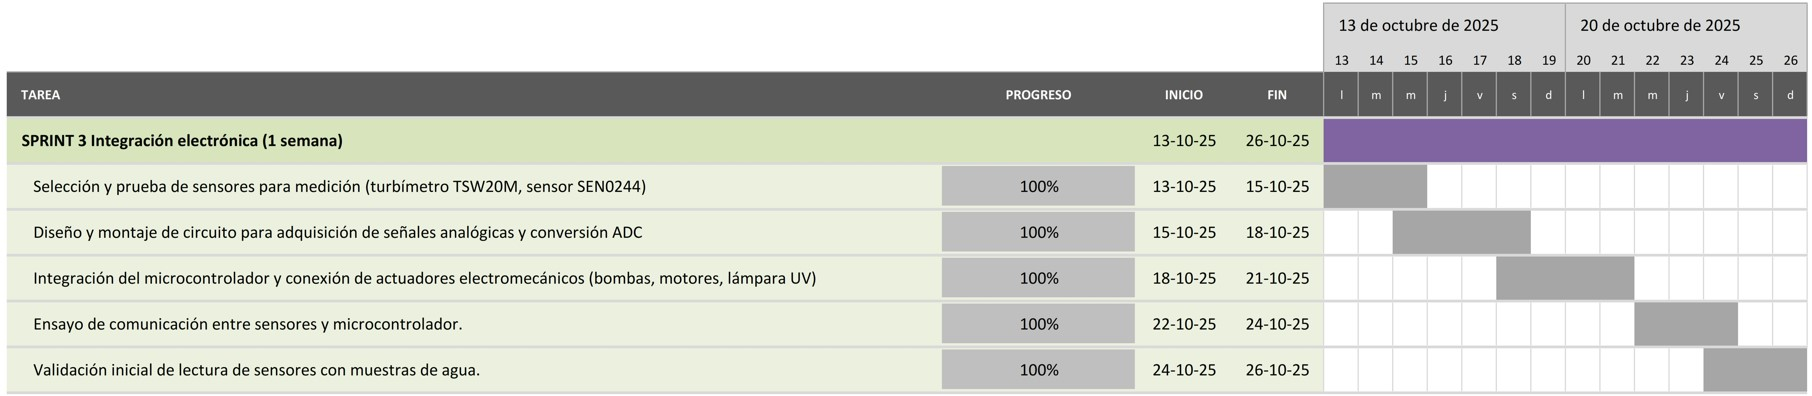
\includegraphics[width=\columnwidth]{fig5_3.jpg}
	%\caption{Implementacion de metricas de alcance}
	%\label{fig:esquema-sistema}
	\end{figure}

	\begin{figure}[!htbp]
	\centering
	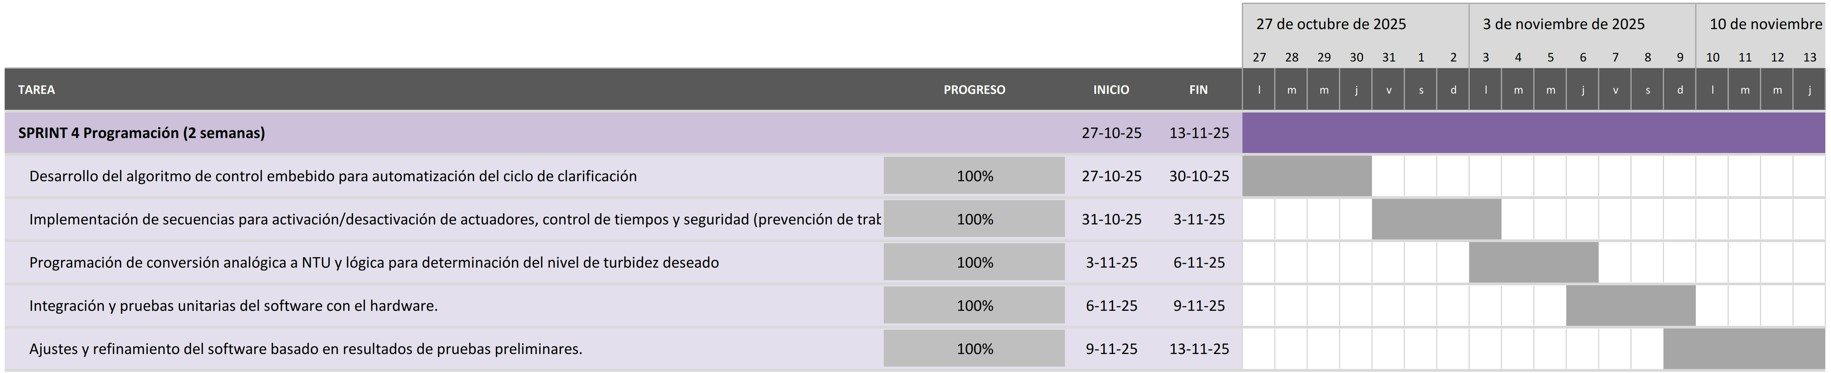
\includegraphics[width=\columnwidth]{fig5_4.jpg}
	%\caption{Implementacion de metricas de alcance}
	%\label{fig:esquema-sistema}
	\end{figure}

	\begin{figure}[!htbp]
	\centering
	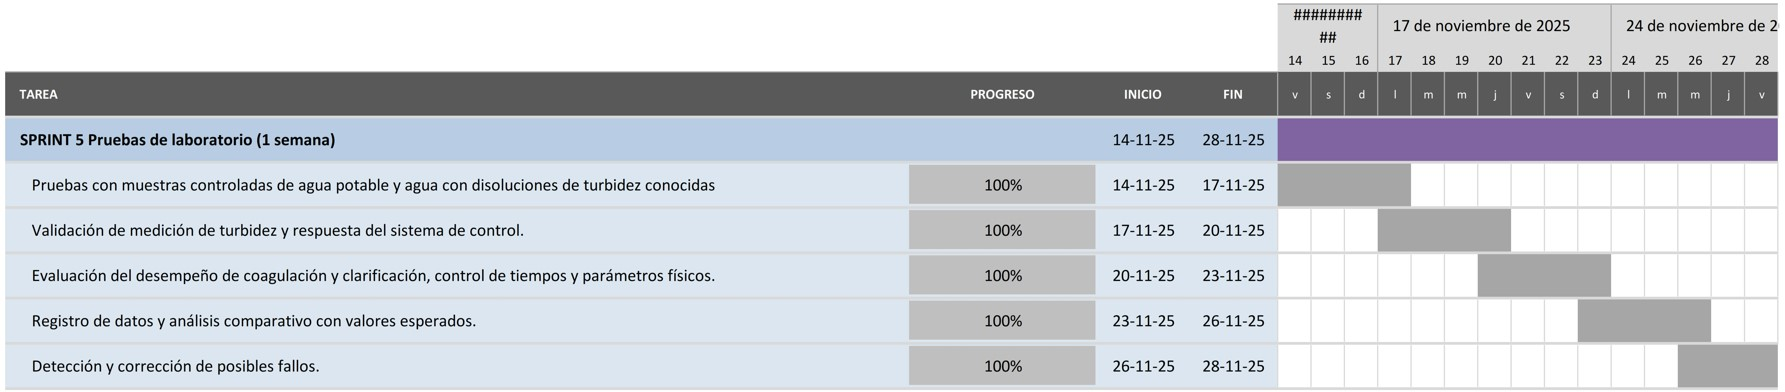
\includegraphics[width=\columnwidth]{fig5_5.jpg}
	%\caption{Implementacion de metricas de alcance}
	%\label{fig:esquema-sistema}
	\end{figure}

	\begin{figure}[!htbp]
	\centering
	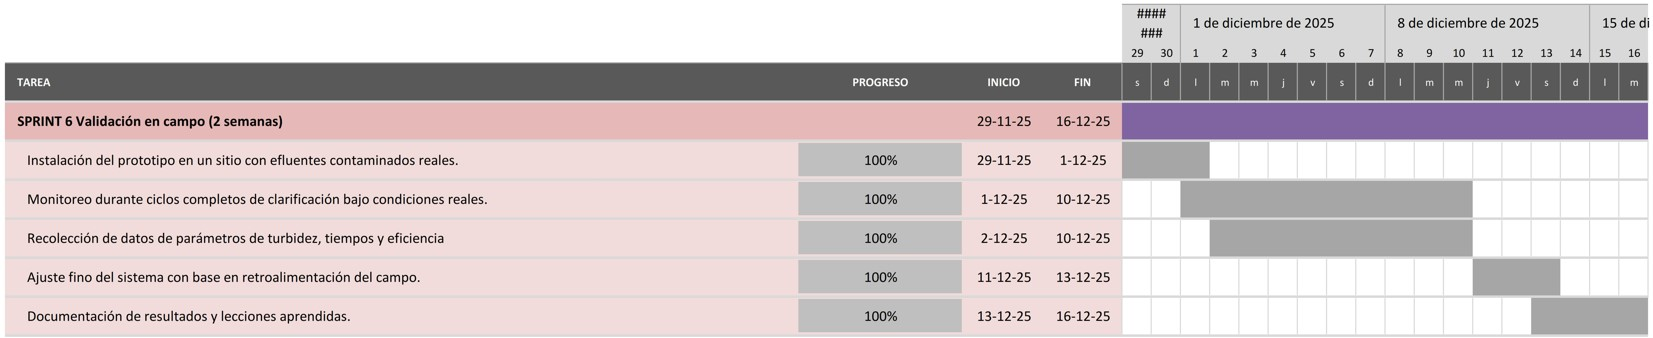
\includegraphics[width=\columnwidth]{fig5_6.jpg}
	%\caption{Implementacion de metricas de alcance}
	%\label{fig:esquema-sistema}
	\end{figure}

	\begin{figure}[!htbp]
	\centering
	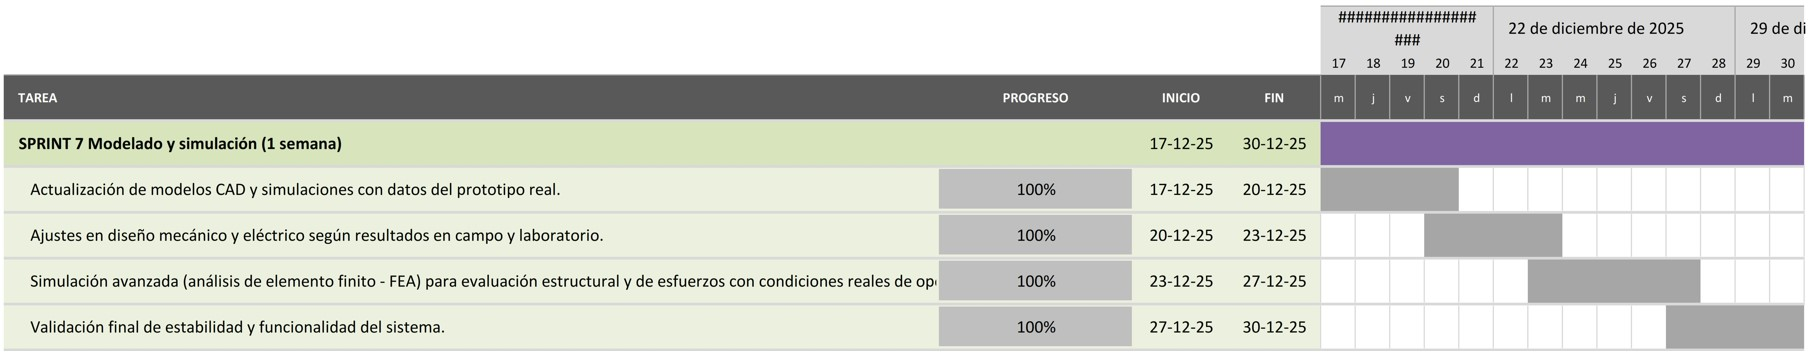
\includegraphics[width=\columnwidth]{fig5_7.jpg}
	\caption{Cronogama de actividades por sprints.}
	%\label{fig:esquema-sistema}
	\end{figure}

	\subsection{MATERIALES Y MÉTODOS}
	
	\subsubsection{Arquitectura del prototipo y sistema embebido}
	
	El dispositivo está estructurado por medio de un conjunto de sistemas mecánicos y eléctricos de potencia que estarán controlados por un sistema embebido, ambos arreglos serán de diseño propio con base en las funciones de operatividad y portabilidad del prototipo, según sea el caso de la aplicación requerida (volumen del efluente, nivel de turbiedad, entre otros) como se muestra en la figura 6.
	
	El sistema se basa en un microcontrolador PIC18F4550, seleccionado por su capacidad de procesamiento, puertos analógicos y comunicación USB. Se integran sensores de turbidez (TSD-10), TDS, pH, temperatura (DS18B20) y nivel (HC-SR04). Los actuadores incluyen motor de agitación, servoválvulas, bomba peristáltica y lámpara UV.
	
	El código fue desarrollado en lenguaje C utilizando MPLAB X IDE. La arquitectura sigue el modelo modular orientado a eventos, con capas de abstracción para sensores, actuadores, lógica de control y comunicación. Se implementaron rutinas de filtrado digital, calibración automática y detección de fallos.
	
	\begin{figure}[htbp]
		\centering
		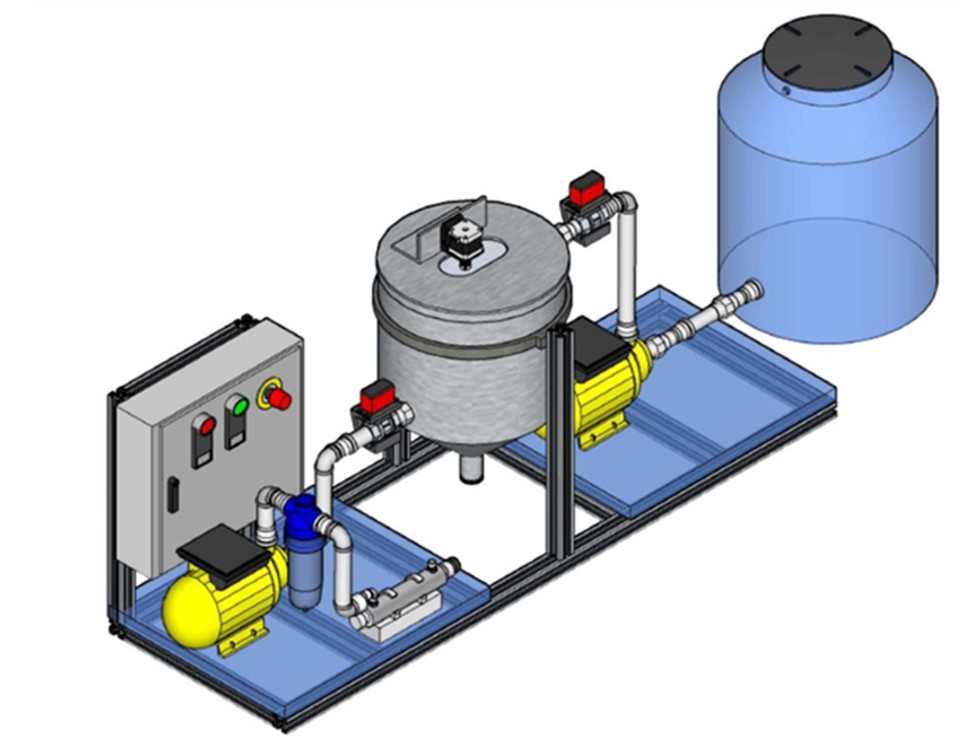
\includegraphics[width=0.9\columnwidth]{fig6.jpg}
		\caption{Modelo isométrico del sistema, proyección sólida.}
		\label{fig:arquitectura-sistema}
	\end{figure}

	Esencialmente lo que procede en el prototipo es la ejecución de cinco etapas de funcionamiento específicas las cuales se establecen de la siguiente forma:
	
	\begin{enumerate}
		\item Etapa de alimentación de efluente tras la verificación de temperatura.
		\item Etapa de dosificación del floculador a partir de la lectura del fluido en el tanque principal.
		\item Etapa de ejecución de la reacción por medio de la activación del agitador.
		\item Etapa de descarga a través de un filtro activo de carbón y desinfección por radiación UV.
		\item Etapa de radiación UV del efluente.
	\end{enumerate}
	
	Esta secuencia de acciones se presenta en la figura 7, las cuales requieren establecer una plataforma de control adecuada y robusta para el prototipo adecuando de forma eficiente los instrumentos de medición para los parámetros referidos de control entre los que figuran en forma específica los valores de temperatura y nivel, como valores de arranque de proceso, así como de turbidez y pH. De esta manera, se generan las activaciones de los sistemas de bombeo de llenado, la aplicación del floculante, el accionamiento del agitador y por último el drenado y purificación final del efluente.
	
	\begin{figure}[htbp]
		\centering
		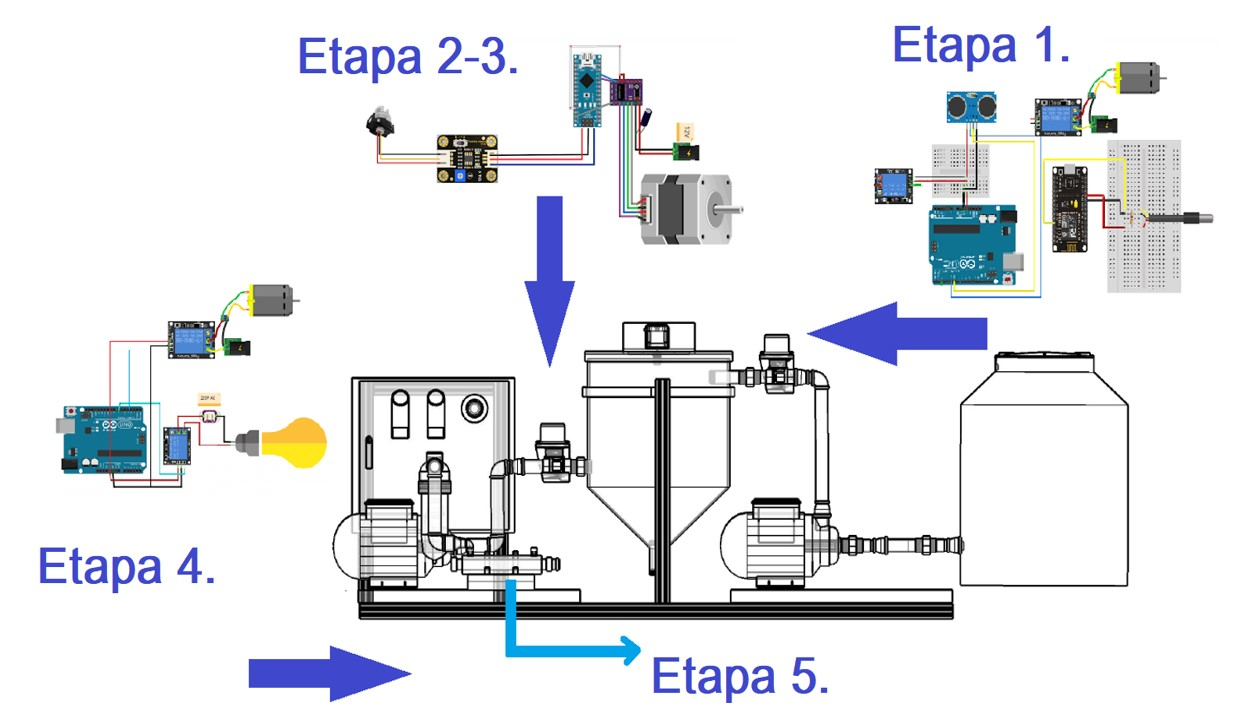
\includegraphics[width=\columnwidth]{fig7.jpg}
		\caption{Esquema del funcionamiento del proceso con base en la disposición del prototipo de planta.}
		\label{fig:secuencia-acciones}
	\end{figure}
	
	Habiendo ya preestablecido la configuración y lógica de operación y control para la planta de proceso ahora se establece una descripción general del algoritmo para su correspondiente codificación. Para la realización del algoritmo se hace uso de un modelo de programación top-down, de forma tal que se trasladan las 5 etapas generales por medio de un diagrama de flujo que permite bosquejar en forma más concreta el algoritmo, para establecer la secuencias y estructuras cíclicas a implementar, de igual forma se definen las variables de entrada y salida, para el diseño de planta, el diagrama de flujo para el diseño, el cual se muestra figura 8.
	
	\begin{figure}[!htbp]
		\centering
		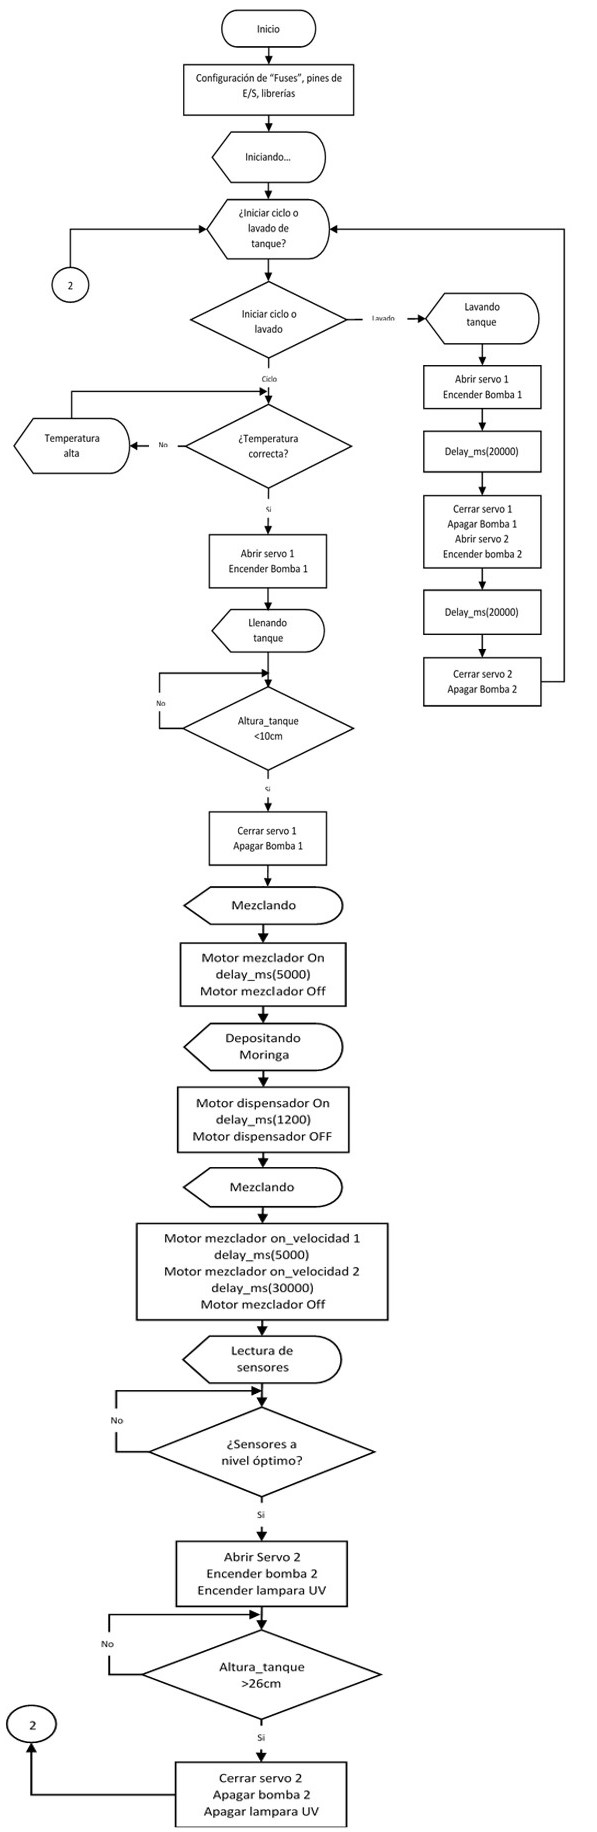
\includegraphics[width=0.6\columnwidth]{fig8.jpg}
		\caption{Diagrama de flujo de operación general del proyecto.}
		\label{fig:secuencia-acciones}
	\end{figure}

	Con el fin de implementar un sistema embebido de diseño propio que se encargue de operar en forma automática el proceso total, activando los diferentes dispositivos de potencia o actuadores con base en la señal de entrada del sensor de medición de nivel, índice de turbiedad detectado y tiempos programados de ejecución, es relevante hacer uso de un microcontrolador de gama media/alta como lo es el PIC18F4550. Este microcontrolador cuenta con 5 puertos E/S, 4 temporizadores, 20 fuentes de interrupción, comunicación serial, modulo USB, 13 canales de entradas analógicas y dos módulos PWM. La distribución de sus pines se puede observar en la figura 9.
	
	\begin{figure}[htbp]
		\centering
		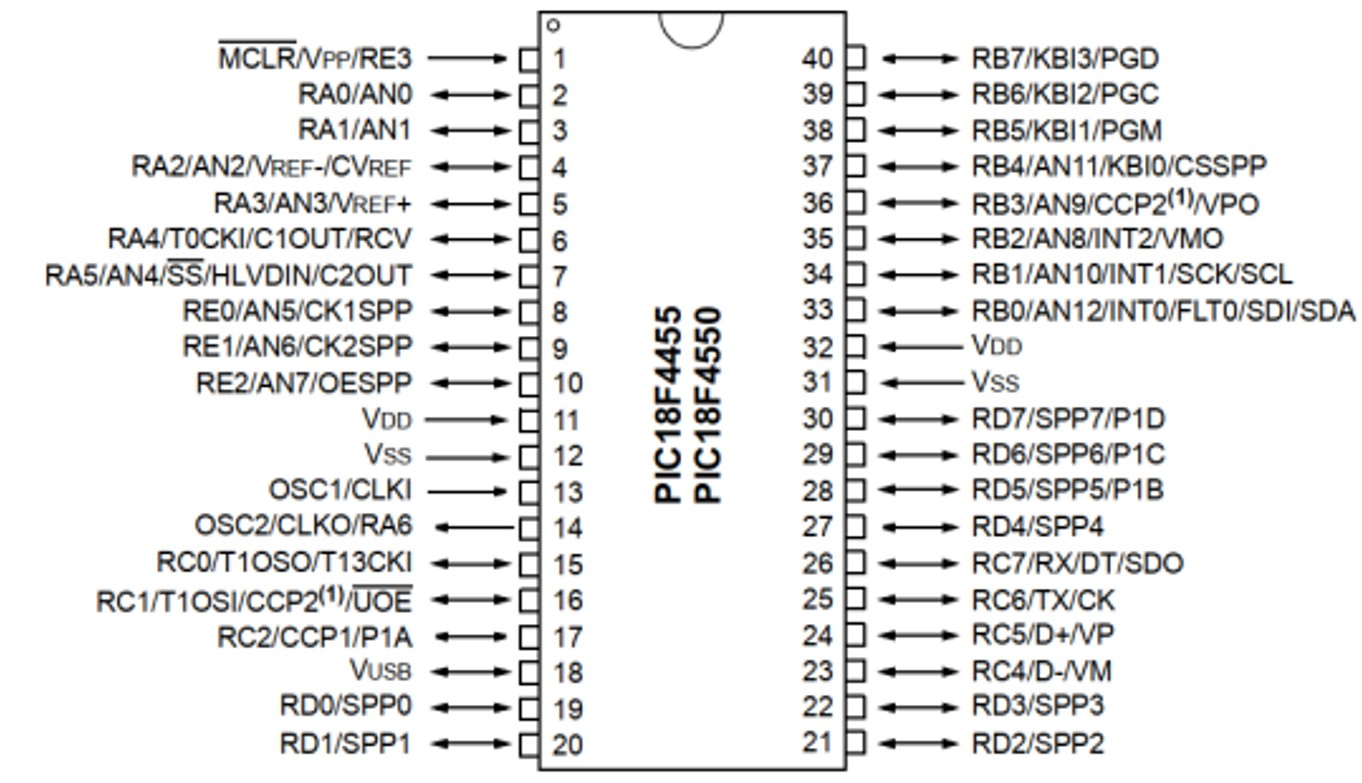
\includegraphics[width=0.6\columnwidth]{fig9.jpg}
		\caption{Esquema de distribución de los pines del PIC18F4550 (Data Sheet, Microchip Technology Inc., USA, 2009).}
		\label{fig:secuencia-acciones}
	\end{figure}
	
	\section{Parámetros de medición del agua.}
	El agua de consumo inocua (agua potable), debe presentar parámetros de calidad, que no ocasione ningún riesgo significativo para la salud cuando se consuma. Esta condición de los recursos hídricos puede definirse, además, como el conjunto de condiciones y medidas necesarias durante la producción, almacenamiento, distribución y preparación del mismo para asegurar que al ingerirse, no representen un riesgo para la salud. Estos parámetros de medición de la calidad del agua están asociados a las características químicas, físicas y biológicas que este líquido debería cumplir, según los valores establecidos para su uso, que son los siguientes:
	
		\begin{itemize}
		\item \textbf{TDS (Total Dissolved Solids):} Total de sólidos disueltos y lo que hacen los lectores de TDS es medir la concentración total de los sólidos disueltos en el agua. Los TDS se componen de sales inorgánicas. Las sales inorgánicas comunes presentes en el agua son los minerales como calcio, magnesio, potasio y sodio, entre otros. Los sólidos totales (TDS) son la suma de todos los sólidos disueltos y suspendidos en el agua. TDS puede ser de las sustancias orgánicas como inorgánicas, los microorganismos y partículas más grandes como la arena y arcilla.
		
		\item \textbf{DBO y DQO:} Los análisis se pueden también hacer por medidas del carbón orgánico total (COT) y por la demanda biológica (DBO) y química de oxígeno (DQO). La DBO es una medida de la materia orgánica en el agua, expresada en mg/l. Es la cantidad de oxígeno disuelto que se requiere para la descomposición de la materia orgánica. La prueba de la DBO toma un período de cinco días. La DQO es una medida de la materia orgánica e inorgánica en el agua, expresada en mg/l es la cantidad de oxígeno disuelto requerida para la oxidación química completa de contaminantes.
		
		\item \textbf{Turbidez:} La turbidez es una medida del grado en el cual el agua pierde su transparencia debido a la presencia de partículas en suspensión. Cuantos más sólidos en suspensión haya en el agua, más sucia parecerá ésta y más alta será la turbidez. La turbidez es considerada una buena medida de la calidad del agua. Este parámetro mide la cantidad de partículas suspendidas en el agua. Su unidad de medida es NTU (unidad nefelométrica de turbidez). La turbidez del agua también reduce la afectividad de desinfección. Los microorganismos pueden quedar protegidos del efecto de los agentes desinfectante por la turbidez de las aguas.
		
		
		\item \textbf{Conductividad:} Mide la capacidad de conducción de corriente eléctrica que tiene el agua, según la cantidad de minerales contenidos en esta. Se mide en microsiemens ($\mu$S) o en Siemens por metro (S/m). No obstante, para usarlo como indicador de calidad habría que analizar el tipo de minerales que contiene. Por ejemplo, el calcio y el arsénico suman al agua una gran capacidad de conductividad, pero el último de estos minerales resulta letal para el consumo, incluso, en valores mínimos de microsiemens. La medida de la conductividad del agua puede proporcionar una visión clara de la concentración de iones en el agua, pues el agua es naturalmente resistente a la conducción de la energía.
			
		\item \textbf{Temperatura:} Al medir la temperatura del agua, se encuentra una relación con el pH y conductividad de esta, por lo tanto, este indicador se mide en conjunto. Su unidad de medida se expresa en Kelvin (K). La temperatura también influye la efectividad de los desinfectantes. El aumento de la temperatura produce un aumento de la velocidad de las reacciones y la desinfección. También puede provocar la volatilización o inactivación del agente desinfectante contra la desinfección del agua.
	
		\item \textbf{Contaminación microbiana:} La contaminación microbiana es dividida en la contaminación por los organismos que tienen la capacidad de reproducirse y de multiplicarse y los organismos que no pueden hacerlo. Este es un parámetro sensible para la evaluación del sistema propuesto. En México se mide este indicador con la unidad de medida CF (formadores de colonias), junto a otros indicadores, para determinar la potabilidad del agua designada para el consumo humano.
	
	\end{itemize}
	
\subsection{Diseño sistema eléctrico}

Todo el proceso se regula por medio de un PIC18F4550. La razón del uso de este microcontrolador es la necesidad de utilizar 25 pines para la conexión de 5 sensores, 2 botones, 7 actuadores y una pantalla LCD (liquid-crystal display). Lo anterior con la siguiente configuración de conexión:

\begin{enumerate}
	\item Sensor de sólidos totales disueltos.
	\item Sensor de turbidez.
	\item Sensor de pH.
	\item Sensor de distancia por ultrasónico.
	\item Servomotores para válvulas de flujo.
	\item Sensor de temperatura.
	\item Microcontrolador.
	\item Pulsadores de arranque y paro con resistencias de pulso alto.
	\item Motores a pasos y sus módulos de control.
	\item Lámpara de radiación UV y su relevador de arranque.
	\item Bombas de flujo y sus relevadores de arranque.
	\item Pantalla de cristal líquido como interfaz de usuario.
\end{enumerate}

Dado lo anterior, se descarta la posibilidad de utilizar el PIC18F2550 que básicamente cuenta con las mismas características que el microcontrolador seleccionado, pero solamente con 21 pines disponibles para entradas y salidas. Así, el PIC18F4550 se encarga de operar en forma automática el ciclo total, activando los diferentes elementos del proceso con base a las señales adquiridas y los tiempos programados de ejecución, lo anterior se muestra en el diagrama de la figura 10.

\begin{figure}[htbp]
	\centering
	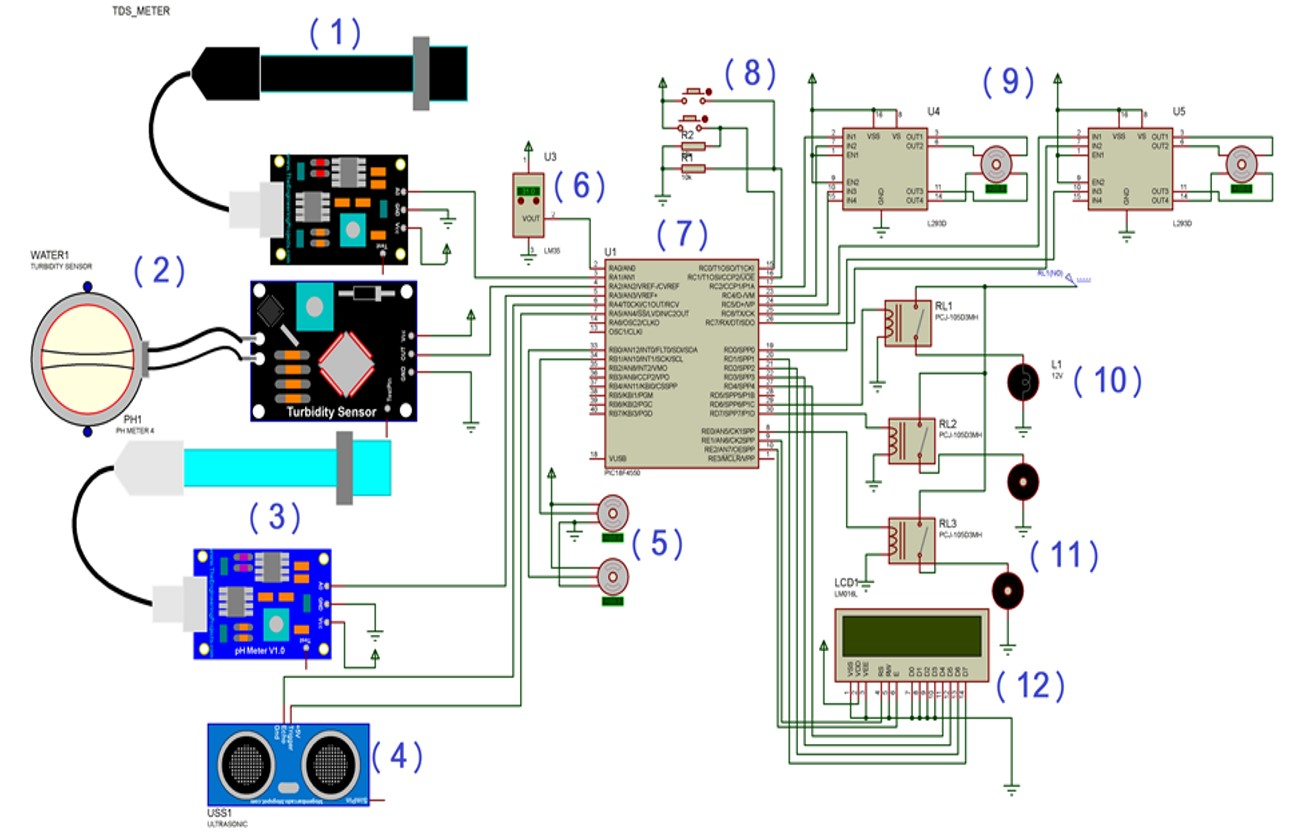
\includegraphics[width=0.8\columnwidth]{fig10.jpg}
	\caption{Arreglo eléctrico del sistema de operación y control}
	\label{fig:arreglo-electrico}
\end{figure}
		
El diseño anterior se estructura como se observa en la figura 11, donde cada uno de los puntos de conexión de salidas y entradas se construyen como un sistema embebido de diseño propio para la aplicación especificada.

\begin{figure}[htbp]
	\centering
	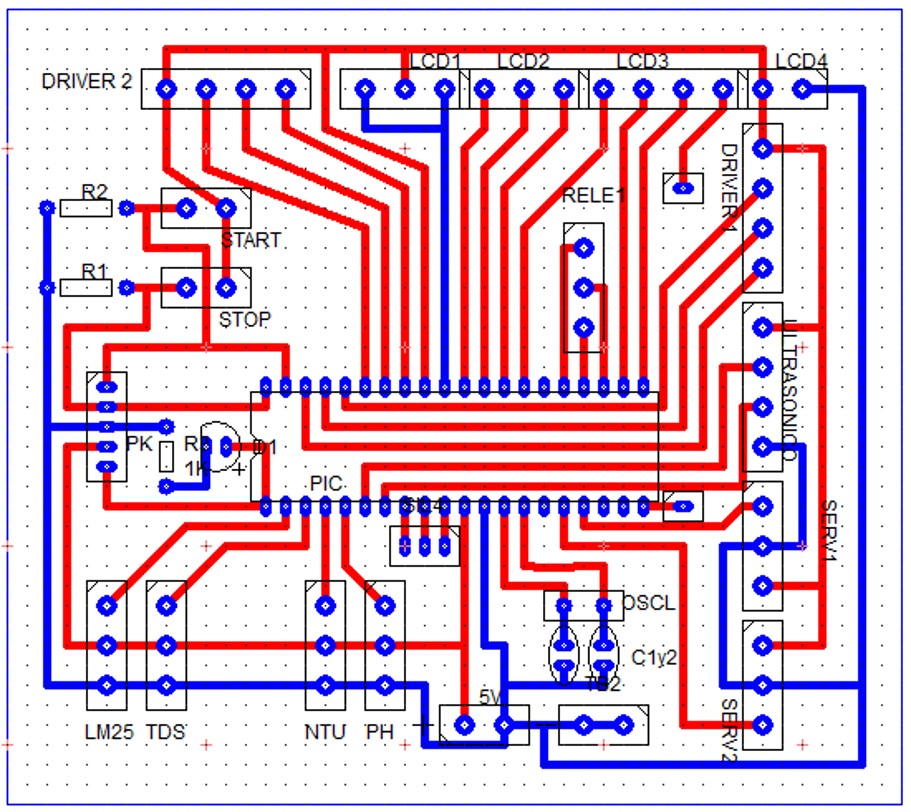
\includegraphics[width=0.8\columnwidth]{fig11.jpg}
	\caption{Esquemático de la tarjeta de control}
	\label{fig:esquematico-tarjeta}
\end{figure}

A partir de lo anterior se presenta la implementación de los sensores fisicoquímicos en el proceso. Las variables elegidas para la medición son, en buena medida parámetros de referencia adecuados para el proceso de potabilización deseado. Estos valores de referencia, se analizaron previamente en la sección introductoria del presente trabajo. A partir de esta metrología para características fisicoquímicas, es factible mantener rangos de control eficaces para la ejecución del proceso, los cuales son:


\begin{itemize}
	\item Turbidez
	\item TDS
	\item pH
	\item Temperatura
\end{itemize}

Cabe mencionar que aunado a estos valores se someterán a análisis los efluentes tratados, por medio de métodos de bioquímica específicos para estos rubros, ya que parámetros como el DQO, DBO son de vital importancia para el aseguramiento de la calidad del producto, tratamiento final y la eficiencia del proceso propuesto, es importante mencionar que los sensores aplicados para los datos fisicoquímicos son de naturaleza analógica.

\subsection{Análisis de turbidez}

El primer parámetro y uno de los principales dada la naturaleza del proyecto propuesto, es el análisis de turbidez. Para medir este valor se debe medir la dispersión de la luz. En presencia de una solución turbia, la cantidad de luz transmitida es muy baja. Es decir, en el lado del receptor, se obtiene solo una luz de baja intensidad y esta intensidad es inversamente proporcional a la turbidez, figura 12.

\begin{figure}[htbp]
	\centering
	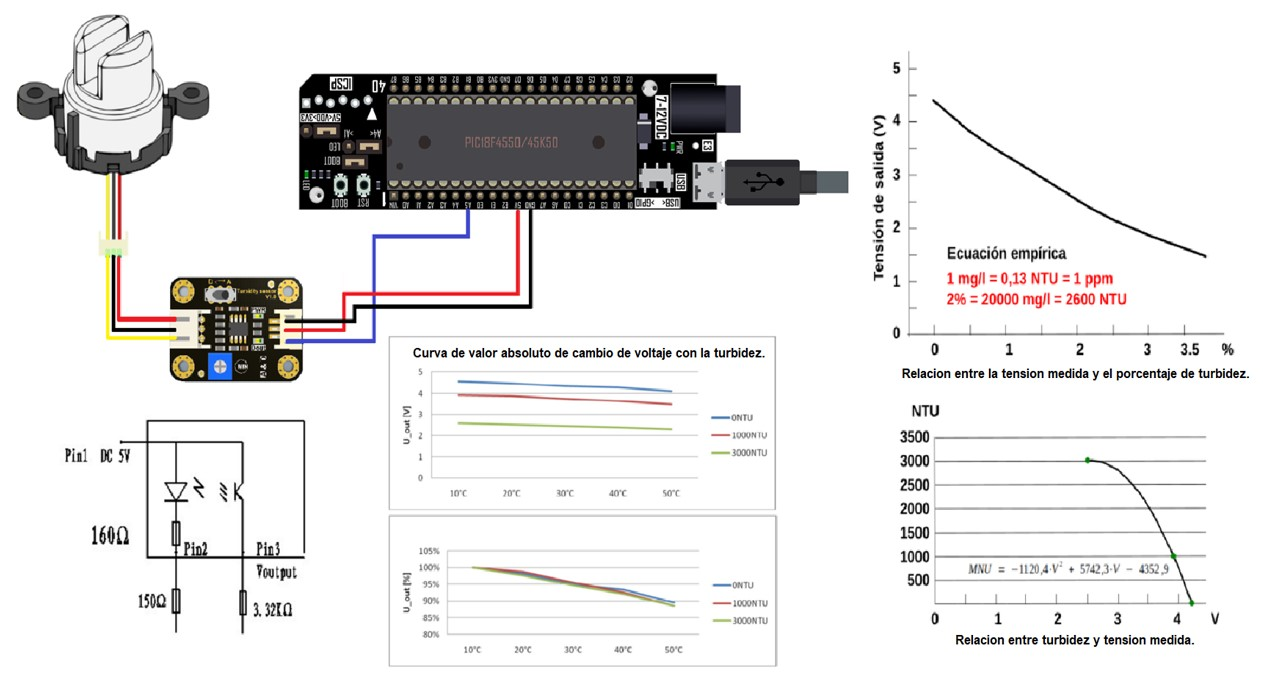
\includegraphics[width=0.9\columnwidth]{fig12.jpg}
	\caption{Estructura interna, esquema de conexión y curvas de lectura para el sensor TSW20M}
	\label{fig:sensor-turbidez}
\end{figure}

	
Con base al análisis indicado se aplica el algoritmo para este sensor, donde la lectura es un parámetro analógico en la que se aplica su conversión con base al principio de conversión analógica digital, para utilizar la curva de variación respecto al voltaje adquirido, se determina el valor en NTU, el algoritmo para generar la adquisición y filtrado de estos datos se muestra en la figura 13.

\begin{figure}[htbp]
	\centering
	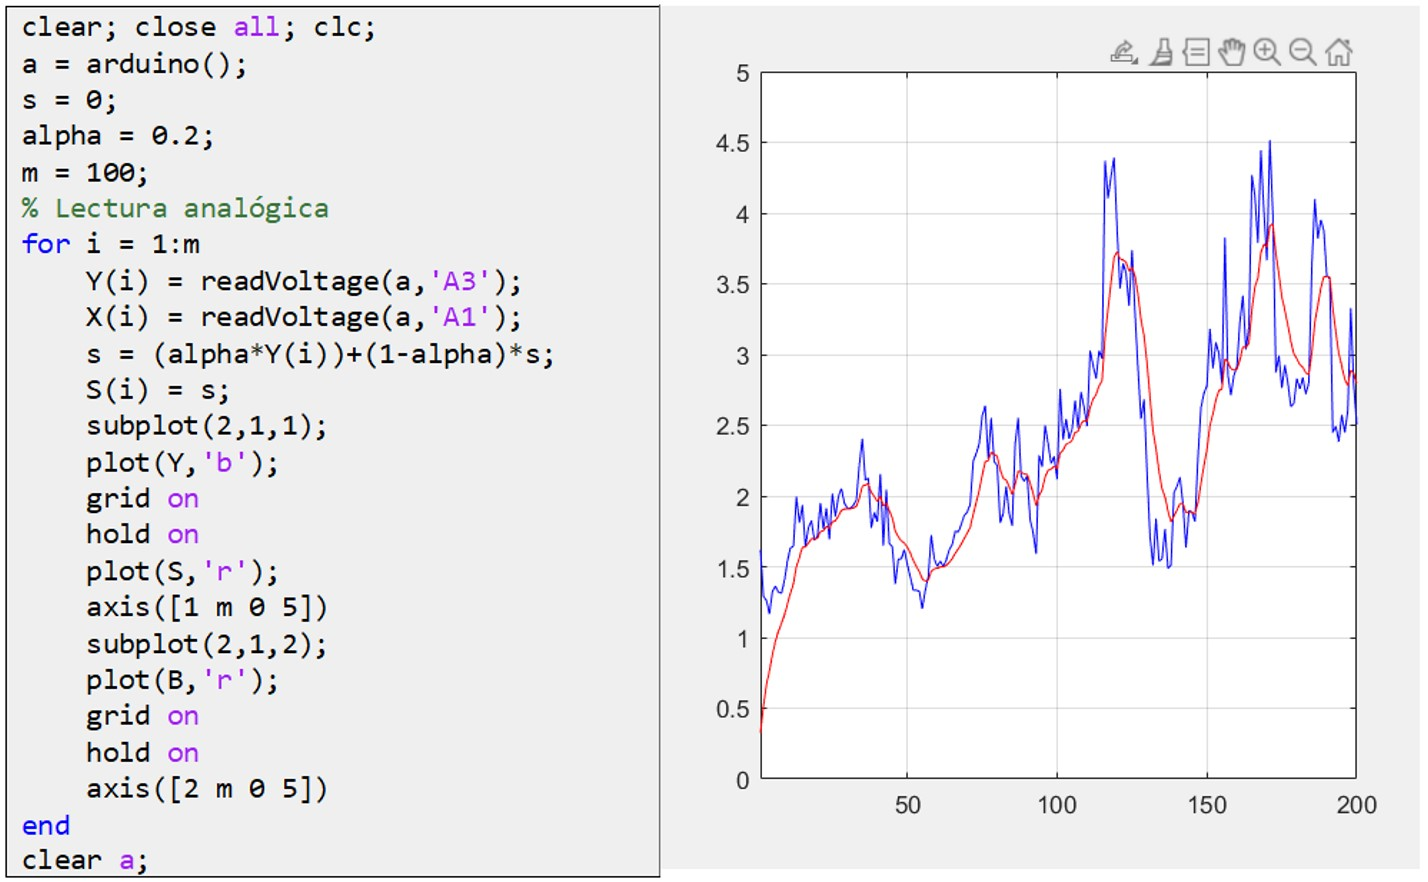
\includegraphics[width=0.8\columnwidth]{fig13.jpg}
	\caption{Código y gráficos de salida para las NTU adquiridas de las muestras}
	\label{fig:codigo-turbidez}
\end{figure}

\subsection{Análisis de TDS}

El TDS es un valor que proporciona un referente de la dureza del agua que pueden generar detrimento en la salud. De esta forma la Organización Mundial de la Salud (OMS) y otras instituciones que regulan la calidad del agua consideran valores hasta los 500 mg/l como completamente seguros, y hasta 1200 mg/l como suficientemente seguros para consumir de manera temporal si no hay otra fuente de agua fácilmente disponible. El principio de funcionamiento de un lector de TDS se basa en la conductividad del agua, al tener en cuenta que todos los sólidos disueltos en el agua tienen cierta carga eléctrica. La medida que el lector utiliza es en PPM (Partes Por Millón). El principio de operación se evalúa en la figura 14.

\begin{figure}[htbp]
	\centering
	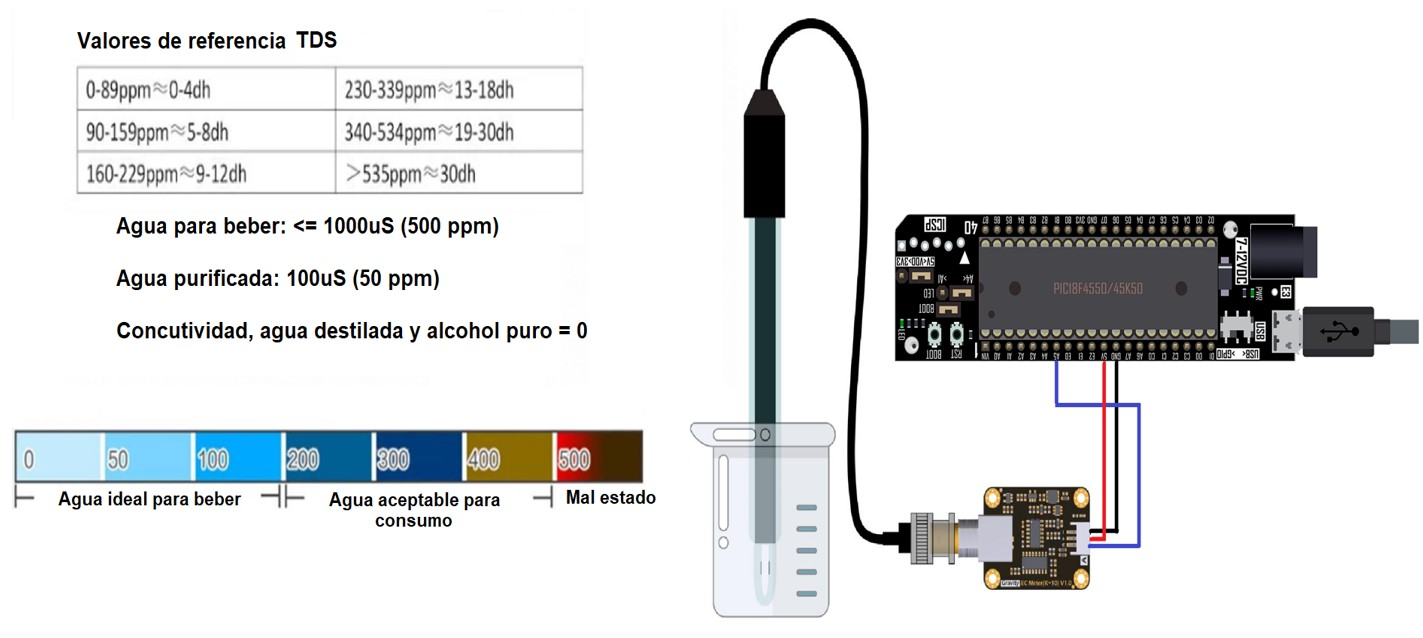
\includegraphics[width=0.8\columnwidth]{fig14.jpg}
	\caption{Datos de referencia y esquemático de conexión para uso del sensor SEN0244}
	\label{fig:sensor-tds}
\end{figure}

Con base en el anterior análisis se procedió a aplicar el código con base a configuración de operación aportado por el fabricante, para de esta forma determinar las mediciones correspondientes para agua de grifo convencional y una muestra de gel antibacterial al 75\% de alcohol. De esta forma, se puede estar en condiciones de medir esta variable en forma continua y en tiempo real, figura 15.

\begin{figure}[htbp]
	\centering
	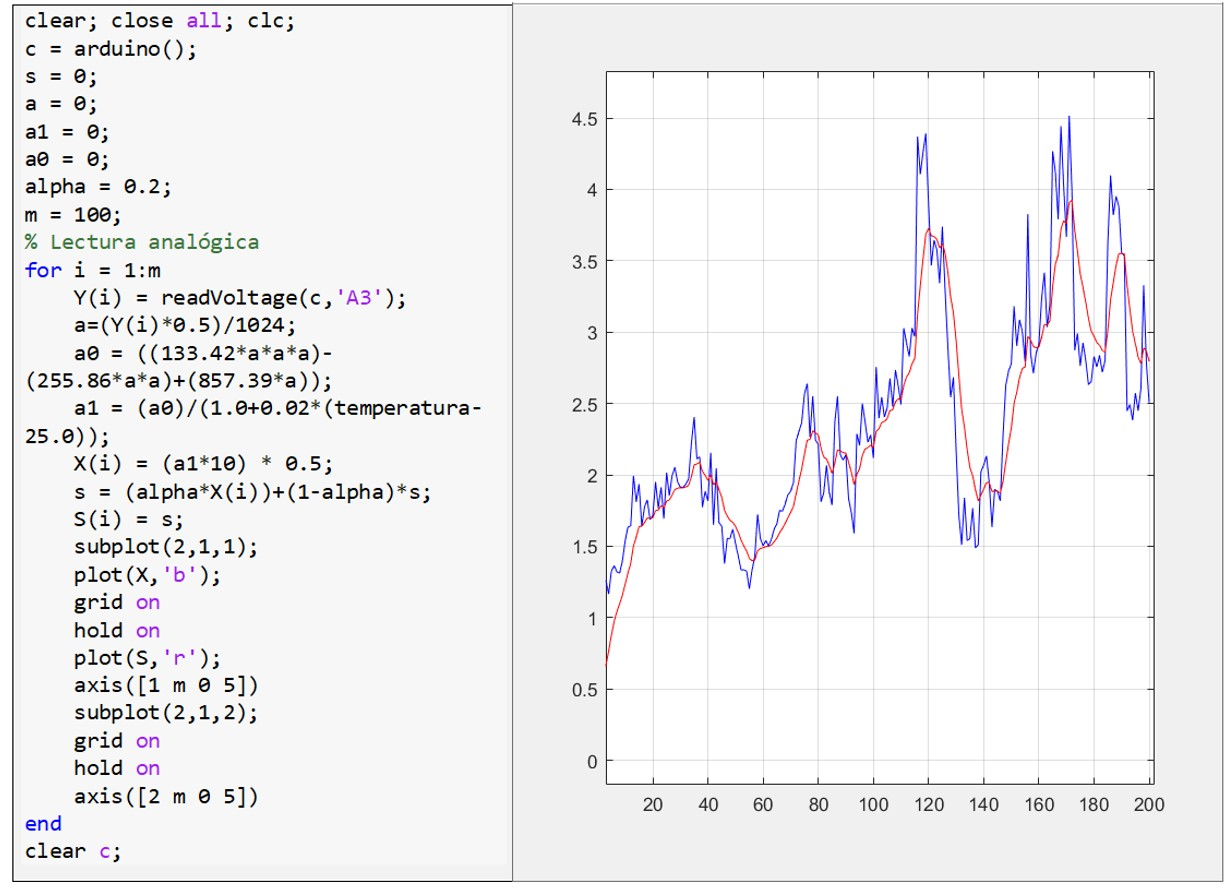
\includegraphics[width=0.8\columnwidth]{fig15.jpg}
	\caption{Código para sensor TDS y resultados adquiridos para muestras de agua corriente y gel a base de alcohol}
	\label{fig:codigo-tds}
\end{figure}

\subsection{Análisis de pH y de temperatura}

Los cambios en pH pueden alterar la concentración de otras substancias en el agua modificando el nivel de toxicidad, por ejemplo: una disminución en el pH puede aumentar la cantidad de mercurio soluble en el agua. Por otra parte, la temperatura es un parámetro físico que afecta a la cantidad de oxígeno que puede transportar el agua, si a la temperatura es alta esta condición favorece a la proliferación de bacterias además de alterar en forma negativa al mecanismo de floculación. De esta forma estas variables son condicionales para la operación del proceso, figura 16.

\begin{figure}[htbp]
	\centering
	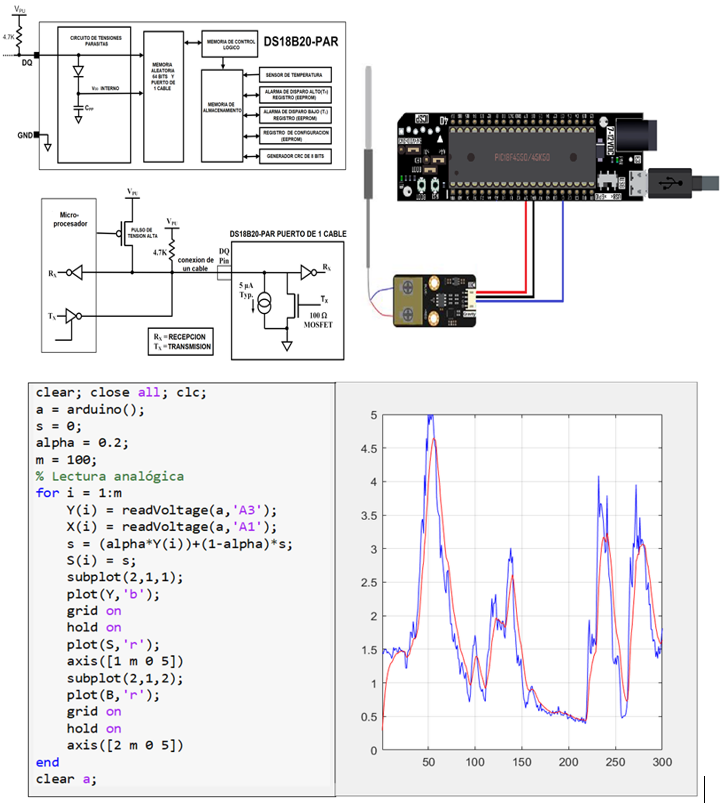
\includegraphics[width=0.9\columnwidth]{fig16.png}
	\caption{Principio de función, conexión y configuración para sensor de temperatura y salida de datos}
	\label{fig:sensor-ph-temperatura}
\end{figure}

Tras la ejecución de estos ensayos, se ha logrado implementar una plataforma de instrumentación para la adquisición de datos de calidad del efluente en tiempo real. Cabe mencionar que se deberán aplicar otros ensayos de calidad el agua, estos deben ser aplicados por el laboratorio con los muestreos que marquen las normativas al respecto y que no son susceptibles de valorarse y evaluarse en tiempo real por lo que no se consideran parámetros de proceso para este prototipo, sin embargo, si de validación y efectividad para el mismo.

\section{Programación del sistema embebido}

Con base en lo antes analizado, se elabora el código en lenguaje C en el programa PIC C Compiler CCS 5.115. En esta primera sección de código mostrado en la figura 17, se procede a establecer la definición y configuración de los puertos, así como la declaración de las bibliotecas necesarias, con la finalidad de establecer los puertos de adquisición de datos para los parámetros fisicoquímicos. De igual manera, se establecen los pines de comunicación para el control de los actuadores.

\begin{figure}[htbp]
	\centering
	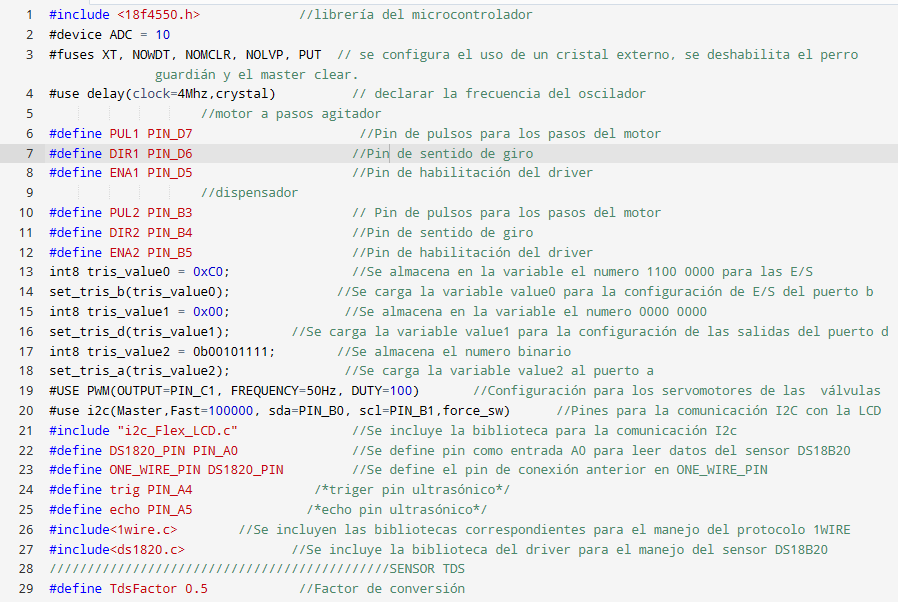
\includegraphics[width=0.9\columnwidth]{fig17.png}
	\caption{Programación del bloque de configuración y bibliotecas de sensores para el PICF18F4550}
	\label{fig:sensor-ph-temperatura}
\end{figure}

Una vez establecida la configuración inicial para la ejecución del algoritmo para el PIC seleccionado, se procede a establecer las rutinas de control. En primera instancia se pregunta si el usuario iniciará el sistema principal o le gustaría realizar una rutina de lavado del tanque, esto es importante puesto que el sedimento queda en el inferior del tanque, este se acumula y debe ser limpiado. Si inicia el sistema principal, la temperatura actuará como un parámetro de inicio, con el fin de asegurar una temperatura adecuada para la acción del floculante, lo anterior queda declarado en el bloque inicial del código principal del algoritmo (figura 18).

\begin{figure}[htbp]
	\centering
	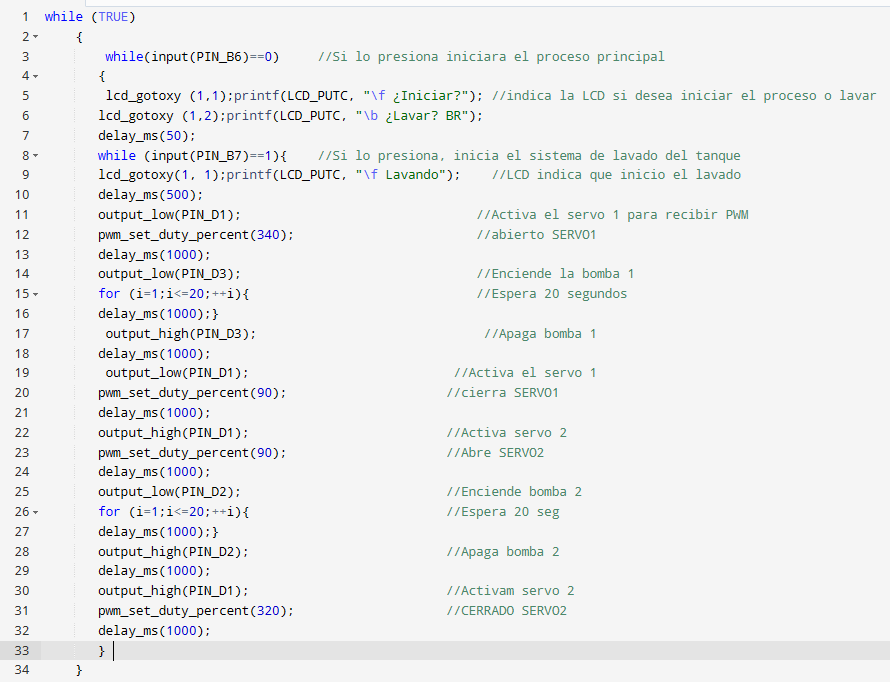
\includegraphics[width=0.9\columnwidth]{fig18.png}
	\caption{Función principal del algoritmo con las instrucciones de interfaz inicial para el usuario}
	\label{fig:sensor-ph-temperatura}
\end{figure}

En este conjunto de instrucciones se agrega también un bloque de sentencias que relaciona el valor de temperatura adquirido por el sensor DS18B20, al presionar el botón de arranque, la lectura deberá cumplir ser inferior a los 28 grados para iniciar el trabajo y abrir la servoválvula de admisión, además de indicar al usuario el mensaje del estado de la temperatura (figura 19). Si no se cumple con la temperatura ideal, esto se indica en la LCD y el programa esperará hasta que se tenga la temperatura adecuada para iniciar la floculación.

\begin{figure}[htbp]
	\centering
	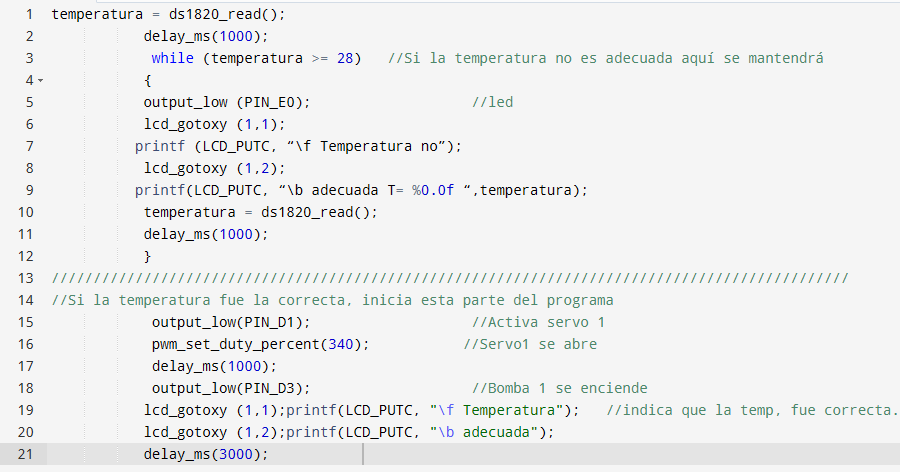
\includegraphics[width=0.9\columnwidth]{fig19.png}
	\caption{Bloque de control para lectura de temperatura.}
	\label{fig:sensor-ph-temperatura}
\end{figure}

Tras ejecutar las rutinas del sistema evalúa, se mide a través del sensor SEN0189, el nivel de turbidez en el efluente, lo anterior en unidades equivalentes con la escala nefelométrica, esto tras el efecto de la acción del coagulante orgánico aplicado. De esta forma, a la lectura analógica recibida, se le aplica una ganancia proporcional, que puede ser en dos formas, por hardware a través de un potenciómetro integrado o a través de la programación de la ganancia respectiva con base a la curva de respuesta del sensor, misma que se analizó en la figura 14. Para el caso particular utilizado, el encapsulado del sensor brinda hermeticidad contra el fluido, sin embargo, limita el acceso al potenciómetro por lo que, tras realizar varios ensayos con diferentes niveles de turbidez, se logró valores eficaces de lectura con el factor de ganancia aplicado.

De forma análoga, también se aplica un factor proporcional de ajuste para el sensor de SEN0244, este instrumento permite adquirir las unidades TDS presentes en el efluente tratado. Cabe mencionar que los dos parámetros son medidos en forma analógica, debido a la naturaleza de los sensores aplicados, por lo que en ambos casos se implementa el algoritmo de conversión para datos analógico-digital.

Finalmente, se aplican las rutinas para la potabilización del efluente, las cuales consisten en la apertura de la servoválvula de salida, así como la activación de las bombas de desfogue y la lámpara de radiación UV. Este último proceso se inicia, con base en el alcance de los parámetros de consigna de las unidades nefelométricas y de sólidos suspendidos. Esta rutina se ve especificada en la sección de código mostrada en la figura 20.

\begin{figure}[htbp]
	\centering
	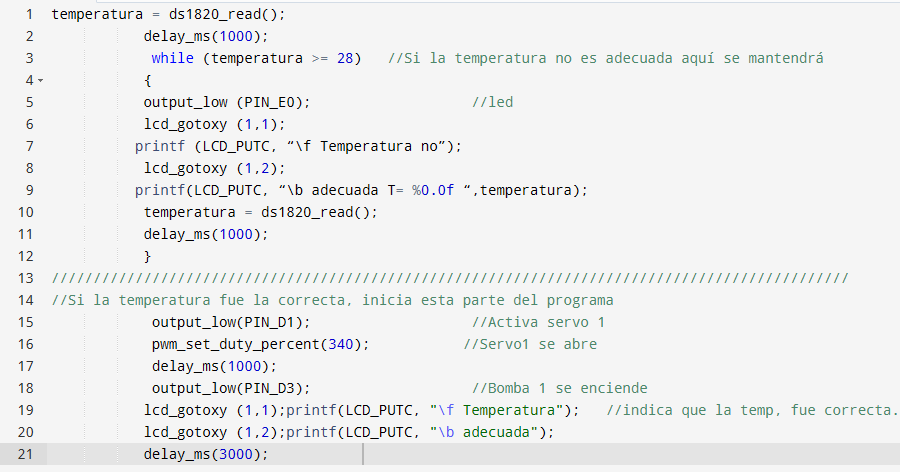
\includegraphics[width=0.9\columnwidth]{fig19.png}
	\caption{Código de etapa de potabilización del efluente, a través de activación de válvula y bomba de salida, así como lámpara UV.}
	\label{fig:sensor-ph-temperatura}
\end{figure}

		
	\begin{thebibliography}{00}
		\bibitem{b1} F. Celis, ``Acceso al agua en M\'exico: la crisis que viene (Forbes),'' Julio 26, 2017. [En l\'{\i}nea]. Disponible en: \url{https://agua.org.mx/acceso-al-agua-en-mexico-la-crisis-viene/}.
		
		\bibitem{b2} E. V\'eliz Lorenzo, J. G. Llanes Oca\~na, L. A. Fern\'andez Garc\'{\i}a y M. Bataller Venta, ``Evaluaci\'on de la eficiencia de los procesos de coagulaci\'on-floculaci\'on y ozonizaci\'on a escala de laboratorio en el tratamiento de aguas residuales municipales,'' \textit{CENIC. Ciencias Qu\'{\i}micas}, vol. 41, no. 1, pp. 49--56, 2010.
		
		\bibitem{b3} R. Devesa-Rey, F. J. Rodr\'{\i}guez-Rodr\'{\i}guez y S. Urr\'ejola-Madri\~nan, ``Dise\~no de un Experimento de Optimizaci\'on del Proceso de Coagulaci\'on-Floculaci\'on Aguas en el Laboratorio de Qu\'{\i}mica,'' \textit{Modelling in Science Education and Learning}, vol. 10, no. 2, pp. 35--43, 2017.
		
		\bibitem{b4} E. d. J. Acevedo Pic\'on, \textit{Uso de semillas de moringa (moringa ole\'{\i}fera) como floculante natural para la purificaci\'on de aguas crudas de rio negro, rio de oro y quebrada Floridablanca, Santander}. Bucaramanga: Universidad de Santander, 2019.
		
		\bibitem{b5} G. Folkard y J. Sutherland, ``Moringa ole\'{\i}fera un \'arbol con enormes potencialidades,'' \textit{Agroforester\'{\i}a en las Am\'ericas (CATIE)}, vol. 8, no. 3, pp. 5--8, 1998.
		
		\bibitem{b6} C. Mu\~noz, ``Floculaci\'on Vital,'' \textit{Induambiente}, no. 161, pp. 80--82, noviembre-diciembre 2019. [En l\'{\i}nea]. Disponible en: \url{https://issuu.com/induambiente1/docs/0-induambiente_ed_161-final}.
		
		\bibitem{b7} D. Acebo-Gonz\'alez y A. T. Hern\'andez-Garc\'{\i}a, ``Los m\'etodos Turbidim\'etricos y sus aplicaciones en las ciencias de la vida,'' \textit{CENIC Ciencias Biol\'ogicas}, vol. 44, no. 1, 2013.
		
		 \bibitem{b8} J. Lugo Mar\'{\i}n, ``Metodolog\'{\i}a SCRUM en la Implantaci\'on de Sistemas de Gesti\'on,'' \textit{Inspenet}, 2024.
		
		\bibitem{b9} BigCode, ``Herramientas de Gesti\'on de Proyectos: JIRA, Trello y M\'as,'' \textit{bigcode.es}, 2025.
		
		\bibitem{b10} SonarSource, ``SonarQube: Herramienta de an\'alisis est\'atico, seguridad y calidad de c\'odigo,'' \textit{sonarsource.com}, 2025.
		
		\bibitem{b11} F. O. Arciniega, ``Modelos y Est\'andares de Calidad (ISO, CMM, CMMI y IEEE),'' Universidad Tecnol\'ogica de Tec\'amac, 2019.
		
		\bibitem{b12} ONU, ``Objetivos de Desarrollo Sostenible: Agua limpia y saneamiento,'' Naciones Unidas, 2020.
		\bibitem{b13} I. Sommerville, Software Engineering, 10th ed. Pearson, 2016.
		\bibitem{b14} IEEE Std 830-1998, IEEE Recommended Practice for Software Requirements Specifications.
		\bibitem{b15} IEEE Std 1540-2001, Standard for Risk Management in System Life Cycle Processes.
		\bibitem{b16} B. W. Boehm, Software Engineering Economics. Prentice-Hall, 1981.
		\bibitem{b17} R. S. Pressman, Ingeniería del Software: Un enfoque práctico. McGraw-Hill, 2010.
		\bibitem{b18} P. Jalote, Software Project Management in Practice. Addison-Wesley, 2002.
		\bibitem{b19} DFRobot, ``Sensor Specifications: Turbidity, pH, TDS,'' 2022.
		\bibitem{b20} Y. Huang, ``3D Printing in Valve Manufacturing,'' Journal of Manufacturing Processes, vol. 35, 2018.
		\bibitem{b21} E. M. Hall, Managing Risk: Methods for Software Systems Development. Addison-Wesley, 1998.
		\bibitem{b22} MathWorks, ``MATLAB and Simulink for Control Systems,'' 2021.
		\bibitem{b23} ISO/IEC 31000:2018, Risk management - Guidelines.
		\bibitem{b24} ISO/IEC 25010:2011, Systems and software engineering - Quality models.
		\bibitem{b25} F. P. Brooks, The Mythical Man-Month. Addison-Wesley, 1995.


		
	\end{thebibliography}
	
\end{document}